% !TeX program = xelatex
% !TeX encoding = UTF-8
\documentclass{MathorCupmodeling}
\let\kaishu\relax
\newCJKfontfamily\kaishu{KaiTi}[AutoFakeBold] %use fake KaiTi
\usepackage{zhlipsum,mwe}%use random characters
\usepackage{mathtools}%use mathtools
\usepackage{amsmath}
\usepackage{siunitx}
\usepackage{graphicx}
\usepackage{enumitem}
\setlist{nosep}

\begin{document}
\begin{center}
{\Large PID}

\end{center}
    \newpage

%-------------------------------------------------------------------

	\section{$PID$控制分析}

\subsection{$PID$介绍}

$PID$控制就是用线性组合的方式,把偏差的比例$P$、积分$I$、微分$D$组合构成控制量。对被控对象展开控制的方法。在$PID$控制器中,通过比例单元$P$将偏差进行比例放大得到输出,但通过这一过程无法消除余差,因此加以积分单元$I$,积分依照偏差累计,只要当偏差不为0时,积分值就不为0,考虑到偏差变化有速度快慢之分,加以微分单元$D$,计算偏差变化的速率,$PID$控制就是综合使用这三个单元来控制被控变量。其原理控制示意以\cref{PID原理}

\subsection{$PID$控制器原理性推导}
	
$PID$控制器是一种线性控制器,其根据给定值$r(t)$与实际输出值$y(t)$构成的控制偏差$e(t)$为:

\begin{figure}[hbpt]
\centering
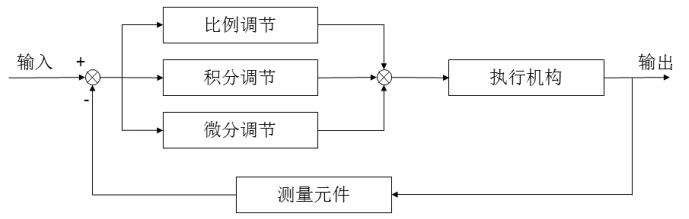
\includegraphics[width=12cm]{PID原理.png}
\caption{PID原理图}\label{PID原理}
\end{figure}

\begin{equation}
e(t)=r(t)-y(t)
\end{equation}

其输入控制偏差$e(t)$与输出控制结果$u(t)$的关系为:

\begin{equation}
u(t)=K_pe(t)+K_I\int_0^te(t)dt+K_D \frac{de(t)}{dt}
\end{equation}

上式进行拉氏变换,得其传递函数为:

\begin{equation}
\begin{aligned}
G(s)&=\frac{U(s)}{E(s)}\\
&=K_p+\frac{1}{K_Is}+K_Ds\\
&=\frac{K(\tau_1s+1)(\tau_2s+1)}{s}
\end{aligned}
\end{equation}

其中,$K_pe(t)$为比例环节,随着$K_p$的增加,可以更好地减小偏差,但同时$K_p$还影响系统的稳定性,$K_p$增加通常导致系统的稳定性下降,过大的$K_p$往往使系统产生剧烈的震荡和不稳定。

$K_I\int_0^te(t)dt$为积分环节,消除系统静态误差,作用的强弱由$K_I$决定,$K_I$越大,积分作用越强,反之则越弱,但同时积分环节也可能增大系统超调量。

$K_D\frac{de(t)}{dt}$为微分环节,针对被测量的变化速率来进行调节,预测偏差信号的变化趋势,在其出现较大变化之前引入修正信号与之低效,从而减小系统的调节时间。

\subsection{实验分析}

实验室倒立摆控制系统结构图如\cref{实验室倒立摆控制系统结构图}

\begin{figure}[hbpt]
\centering
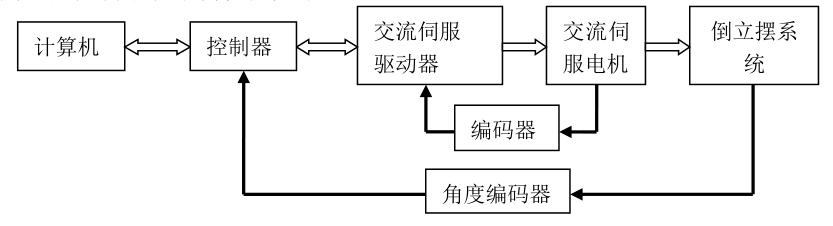
\includegraphics[width=12cm]{实验室倒立摆控制系统结构图.png}
\caption{实验室倒立摆控制系统结构图}\label{实验室倒立摆控制系统结构图}
\end{figure}

修改$PID$各项参数,通过角度编码器测量摆杆的摆动角度,通过伺服电机控制小车的位移速度和加速度,通过控制器利用摆杆的惯性力控制摆杆的位移速度和加速度,从而控制摆杆的角度,最终可以实现直线倒立摆的竖直稳定.

当其受到外界干扰时,在干扰停止作用后,系统能够很快地回到平衡位置。但是,整个控制系统中并无小车位移的反馈,只能通过角度编码器获取摆杆的角度,通过传动比转换近似得到小车的位移。因此 PID控制器无法对小车的位置偏差进行修正,不能对小车的位置进行控制,当受到扰动时,小车会沿滑轨一直向扰动方向运动,撞到滑轨边缘,无法恢复到初始平衡位置。后续考虑使用其它控制方法,既能实现直线倒立摆的竖直稳定,又可以控制小车位置的稳定不变。

\end{document}